\chapter{Plano de Trabalho} \label{cha:plano}


\section{Descrição do Problema}

A instituição financeira objeto deste projeto pretende expandir seu portfólio de produtos por meio de oferta de crédito rural a clientes do agronegócio. No entanto, diferentemente do crédito convencional — onde a análise de risco dos solicitantes é relativamente padronizada por meio de \textit{bureaus} de crédito nacionais (Serasa Experian, Boa Vista SCPC, SPC Brasil, etc.) e de históricos comportamentais internos —, o crédito rural apresenta uma avaliação de risco distinta, governada por diferenças significativas de estrutura das operações e influências externas, como condições climáticas, safras, preços de commodities, entre outros fatores.

As principais fontes de complexidade que caracterizam o problema são:
\begin{itemize}
    \item[(i)] \textbf{Assimetria de informações:} a instituição não dispõe de dados históricos interno no segmento rural e, portanto, não possui padrões de risco comportamental calibrados para essa população;
    \item[(ii)] \textbf{Volatilidade agrícola:} a renda proveniente de atividades agrícolas é dependente de fatores climáticos (regime de chuvas, temperatura, geadas, secas, etc.), de ciclo de preços de \textit{commodities} e de características específicas de cada atividade agropecuária;
    \item[(iii)] \textbf{Heterogeneidade regional:} o Brasil possui dimensões continentais com realidades muito distintas em termos de clima, solo e outros fatores que influenciam a produção agropecuária, gerando perfis de risco diferenciados que modelos genéricos podem apresentar dificuldades para capturar;
    \item[(iv)] \textbf{Especificidade regulatória:} o crédito rural é submetido a um arcabouço normativo com regras específicas de taxas de juros, subvenções e programas de seguro (Proagro) que influenciam o comportamento de inadimplência e devem ser considerados na modelagem de risco.
\end{itemize}

Essas características tornam o desafio de modelar o risco de crédito rural mais complexo. O desafio central do projeto é, portanto: \textbf{\textit{Como construir um modelo preditivo de risco de crédito aplicável à originação de crédito rural, em um contexto de ausência de dados comportamentais próprios, utilizando microdados regulatórios públicos do SICOR/Bacen como fundamento analítico?}}

\section{Hipóteses}

A partir da descrição do problema, formulam-se as seguintes hipóteses de trabalho:
\begin{itemize}
    \item[\textbf{H1:}] A taxa de inadimplência das operações de crédito rural varia significativamente entre atividades agropecuárias, finalidades do financiamento e safras, refletindo a influência diferencial de eventos climáticos e de ciclos de mercado sobre o perfil de risco de crédito de cada segmento.
    \item[\textbf{H2:}] Um modelo preditivo de risco de crédito construido a partir de microdados do SICOR, enriquecidos com variáveis macroeconômicas, setorias e climáticas externas apresenta capacidade preditiva e discriminatória estatisticamente superior a um modelo de referência baseado exclusivamente em taxas históricas de inadimplência.
\end{itemize}

O teste dessas hipóteses fornecerá evidências empíricas sobre a estrutura do risco de crédito rural no Brasil e sobre a viabilidade científica do modelo agnóstico proposto, contribuindo tanto para os objetivos de negócio da instituição quanto para o conhecimento em relação à finanças agrícolas.

\section{Objetivos}

\subsection{Objetivo Geral}

Desenvolver um ecossistema de Business Intelligence e Analytics e um modelo preditivo agnóstico de risco de crédito rural, fundamentado em microdados públicos do Sistema de Operações do Crédito Rural e do Proagro (SICOR/Bacen), capaz de subsidiar a tomada de decisão para apoiar a originação de crédito rural em uma instituição financeira em fase de entrada no mercado, superando os desafios de ausência de dados comportamentais internos e complexidade do ambiente agrícola.

\subsection{Objetivos Específicos}

\begin{itemize}
    \item[\textbf{OE1:}] Construir um pipeline de dados robusto e escalável para ingestão, processamento e análise de microdados do SICOR, integrando fontes de dados externas relevantes (climáticas, macroeconômicas, setoriais) para enriquecer a base analítica.
    \item[\textbf{OE2:}] Realizar uma análise exploratória detalhada dos dados do SICOR para identificar padrões, tendências e relações entre variáveis que influenciam o risco de crédito rural, com foco em segmentação por atividade agropecuária, finalidade do financiamento, safra de originação, região geográfica, etc.
    \item[\textbf{OE3:}] Desenvolver e validar um modelo preditivo de risco de crédito rural utilizando técnicas de aprendizagem de máquina, comparando seu desempenho preditivo e discriminatório com um modelo de referência baseado em taxas históricas de inadimplência.
    \item[\textbf{OE4:}] Criar um dashboard interativo de Business Intelligence para visualização e monitoramento dos indicadores de risco de crédito rural, permitindo a análise dinâmica por diferentes segmentos e facilitando a tomada de decisão para a originação de crédito.
\end{itemize}

\section{Atividades e Cronograma}

O projeto está estruturado com atividades alinhadas aos objetivos específicos, com um cronograma previsto para execução ao longo de três meses (abril a junho de 2026):

\begin{itemize}
    \item[(i)] Revisão bibliográfica e definição do framework analítico;
    \item[(ii)] Extração dos dados do SICOR e avaliação da qualidade dos dados;
    \item[(iii)] Design e implementação do pipeline de ingestão e processamento dos dados (ETL/ELT);
    \item[(iv)] Análise exploratória dos dados (EDA) — originação, volumes, inadimplência por atividade e safra, etc.;
    \item[(v)] Integração de variáveis externas (climáticas, macroeconômicas, setoriais) para enriquecimento da base analítica;
    \item[(vi)] Desenvolvimento e treinamento do modelo de risco de crédito;
    \item[(vii)] Validação e comparação do modelo preditivo com o modelo de referência;
    \item[(viii)] Construção dos dashboards de BI (panorama de originação e risco);
    \item[(ix)] Síntese dos resultados, elaboração do relatório final e apresentação executiva dos resultados.
\end{itemize}

\begin{table}[]
    \caption{Cronograma de Atividades para 2026.}
    \label{tab:cronograma}
    \centering
    \begin{tabular}{c|c|c|c}
        Atividade & Abril & Maio & Junho  \\ \hline
         & & & \\ \hline
         1 & \checkmark &  & \\ \hline
         2 & \checkmark &  & \\ \hline
         3 & \checkmark & \checkmark & \\ \hline
         4 & & \checkmark & \\ \hline
         5 & & \checkmark & \checkmark\\ \hline
         6 & & \checkmark & \checkmark\\ \hline
         7 & & \checkmark & \checkmark\\ \hline
         8 & & & \checkmark\\ \hline
         9 & & & \checkmark\\ \hline
    \end{tabular}
\end{table}

\section{Metodologia}

A metodologia deste projeto segue uma abordagem quantitativa, estruturada em cinco etapas principais:

\subsection{Etapa 1: Coleta de Dados}

Os microdados públicos do SICOR/Bacen serão extraídos diretamente do portal de Dados Abertos do Bacen, cobrindo a série histórica disponível (2013-até o momento). As tabelas relevantes incluem: operações de crédito rural (origem, atividade, finalidade, volume financiado, região, etc.) e registro de pagamentos (inadimplência, datas de vencimento, etc.). De forma complementar, serão coletadas variáveis externas de fontes como IBGE-SIDRA (área plantada, produtividade), Bacen-SGS (taxa Selic, PIB) e CEPEA-Esalq/USP (preços de commodities).

\subsection{Etapa 2: Pipeline de Processamento de Dados}

Um pipeline de processamento será implementado compreendendo:
\begin{itemize}
    \item[(i)] extração dos dados brutos do SICOR e das fontes externas;
    \item[(ii)] transformação, com padronização de chaves de integração, tratamento de dados faltantes, codificação de variáveis categóricas, etc.;
    \item[(iii)] carga em um ambiente de analítico estruturado (data warehouse ou data lake).
\end{itemize}
O pipeline será desenvolvido em Python (cudf, DuckDB), documentado e versionado com Git, seguindo boas práticas de engenharia de dados para garantir reprodutibilidade e escalabilidade.

\subsection{Etapa 3: Análise Exploratória de Dados (EDA)}

Estatísticas descritivas serão calculadas para as principais variáveis de interesse. Será realizado também um diagnóstico do panorama de originação e inadimplência por segmento (atividade, finalidade, safra, região). Visualizações gráficas (histogramas, boxplots, mapas de calor, etc.) serão utilizadas para identificar padrões e relações entre variáveis. A análise de correlação e testes estatísticos serão aplicados para avaliar associações significativas.

\subsection{Etapa 4: Modelagem Preditiva de Risco de Crédito}

A variável-alvo (binária: 0 = adimplente; 1 = inadimplente) será construida a partir dos registros de inadimplência no SICOR. Os modelos preditivos serão estimados em sequência crescente de complexidade, iniciando pelo modelo de referência (\textit{Naïve} baseado em taxas históricas) de inadimplência e finalizando com o modelo de aprendizado de máquina utilizando regressão logística com \textit{feature engineering} e \textit{feature selection} a partir das variáveis do SICOR e das fontes externas. A seleção e avaliação dos modelos seguirão validação cruzada com estratificação por safra agrícola, para garantir a generalização temporal e evitar \textit{data leakage}. O desempenho dos modelos será avaliado por meio das métricas de Área sob a Curva ROC (AUROC), estatística KS (\textit{Kolmogorov-Smirnov}), \textit{Brier Score} e curvas de calibração. A interpretabilidade do modelo será analisada através dos coeficientes da regressão logística (betas), avaliando a influência de cada variável no risco de crédito rural.

\subsection{Etapa 5: Desenvolvimento dos Dashboards de BI}

Os resultados estruturados serão apresentados em dashboards interativos abrangendo:
\begin{itemize}
    \item[(i)] painel de originação, com indicadores de volume financiado, número de operações, tendências por segmento, etc.;
    \item[(ii)] painel de risco, com indicadores de inadimplência por segmento, distribuição de risco, etc.
    \item[(iii)] \textit{output} de \textit{scoring} do modelo de risco.
\end{itemize}
Os dashboards serão desenvolvidos utilizando a biblioteca Streamlit, com Python, com camadas de navegação e filtros para análise dinâmica por diferentes segmentos (atividade, finalidade, safra, região, etc.). O código dos dashboards será documentado e versionado para garantir reprodutibilidade e manutenção futura.

\section{Desenho da Solução}

\begin{figure}
    \centering
    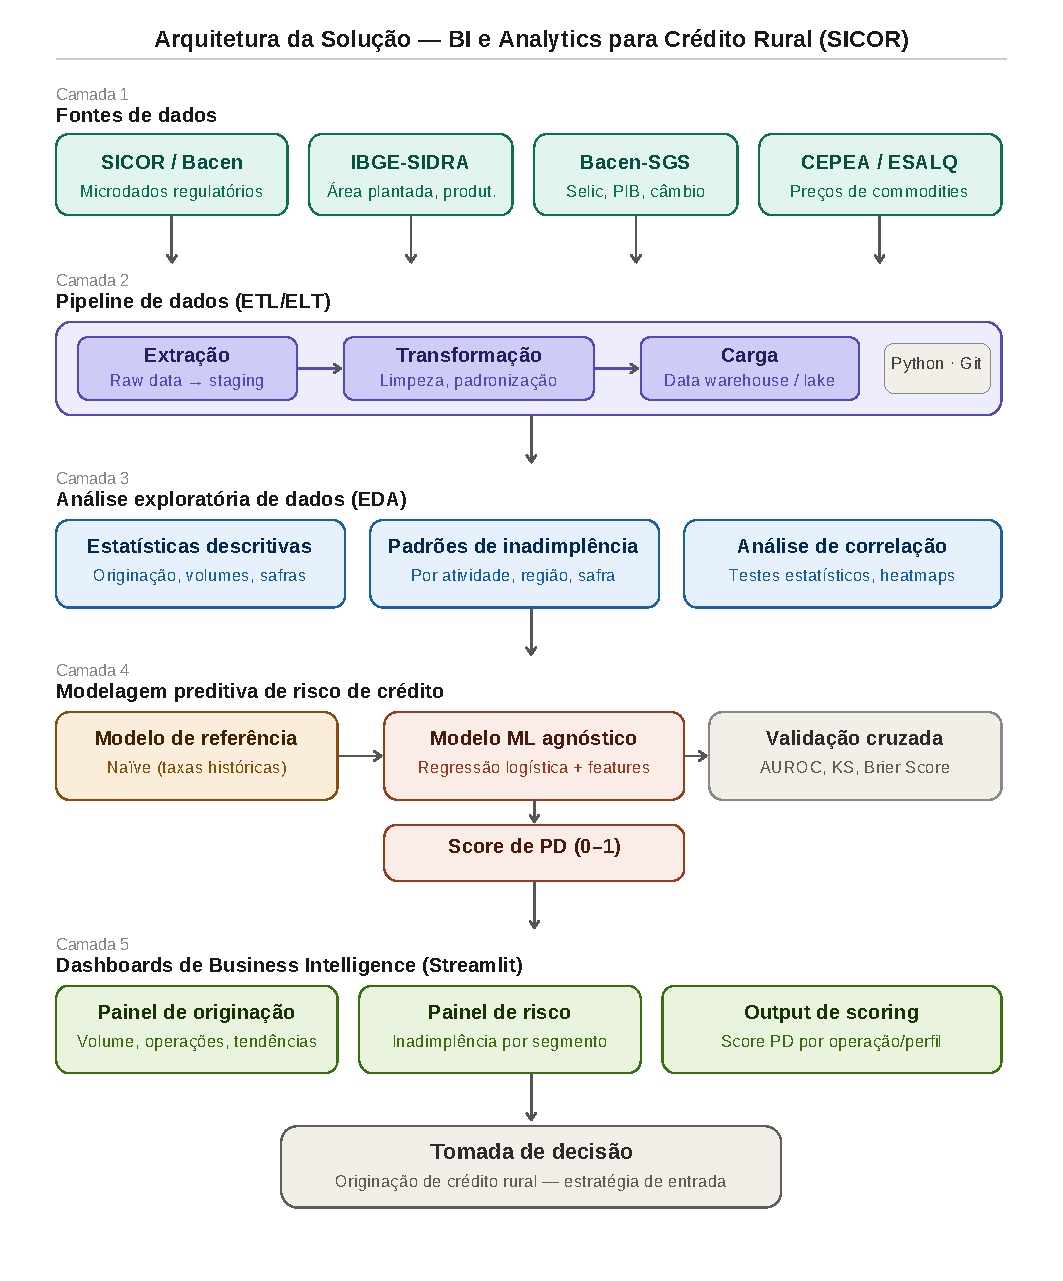
\includegraphics[scale=0.9]{fig/arquitetura_solucao_bi_credito_rural.pdf}
    \caption{Desenho da Arquitetura da Solução}
    \label{fig:desenho-solucao}
\end{figure}

A arquitetura conceitual da solução proposta segue um modelo de camadas progressivas, desde a ingestão dos dados brutos até a entrega do BI para os usuários finais, conforme ilustrado na Figura \ref{fig:desenho-solucao}.

O fluxo de dados percorre as cinco camadas de forma sequencial e rastreável, com as fontes regulatórias e setoriais sendo ingeridas, armazenadas em seu formato bruto. Posteriormente, os dados são processados e transformadas em uma base analítica estruturada, para então serem integrados a modelagem dimensional dos dados. A camada de modelagem opera sobre os dados tratados para produzir as probabilidades de \textit{default} e, por fim, estes serão disponibilizados em dashboards de BI para análise e tomada de decisão. O design modular da arquitetura garante que cada camada possa ser desenvolvida, testada, mantida e atualizada de forma independente, promovendo a escalabilidade e a flexibilidade da solução ao longo do tempo.
